% !TeX spellcheck = en_GB
%Introduction
%\begin{savequote}[50mm]
%If our brains were simple enough for us to understand them, we'd be so simple that we couldn't.
%\qauthor{Ian Stewart }%The Collapse of Chaos: Discovering Simplicity in a Complex World
%\end{savequote}
\chapter{Scope of the research}
\label{chap:introduction}

\section{Motivation}\label{motivation}
We are currently witnessing a transformation of the audio-visual sector towards a new hybrid TV ecosystem, where broadcast and broadband services coexist \cite{Claudy2012}. Although TV continues being the central device for audiovisual media consumption, the proliferation of devices such as mobiles, tablets and laptops together with the supply of Internet capabilities to TV sets, has entailed considerable changes in media production, distribution and consumption \cite{Obrist2015}\cite{McGill2015}. This hybrid ecosystem opens a door to enhance traditional TV shows towards innovative TV experiences, moulding themselves to the new consumption habits and patterns of the users. TV viewers are no longer focused on a single content source or device. They look for additional content on a second screen and they socially interact with friends and the community, related or not to the mainstream media. Furthermore, users are getting used to a multi-device content access, demanding services at any time and from any device \cite{Eastman2012}. Consequently, the consumption of audiovisual and TV programmes has evolved, from viewing them in a stand-alone device to a multi-platform environment, being complemented by websites, applications, online-video streaming, chat rooms and so on.  

\textit{Hybrid TV} and \textit{multi-screening} concepts are linked to multi-platform environments \cite{Bauman2016} and they differentiate TV developments between two segments. Hybrid TV is seen as a concept addressing technologies such as IPTV \cite{iptv} \cite{iptvieee}, OTT-TV \cite{Bauman2016} and HbbTV \cite{hbbtvWeb}, while multi-screening mainly refers to customer behaviour. The latter involves second-screening for related activities, dual screening for unrelated activities and social TV for social networks related activities. The ensemble of both concepts increases the choice offered and TV viewers are expected to switch from a passive form of TV consumption towards an interactive and online multi-screen experience. In addition, traditional broadcasters are trying to adapt their business to these new viewing habits through Broadcast-broadband (or Broadcast-Internet)\footnote{From this point either Broadcast-broadband or Broadcast-Internet terms will be used equally} services.

Figure \ref{fig:hybrid} is extracted from the novel hybrid TV ecosystem analysis in \cite{thesisMikel}, which is an extension of the one depicted by \cite{Claudy2012}. It shows the general overview of the hybrid TV and multi-device experiences and represents the coexistence of the broadcast and broadband channels. On the one hand, traditional broadcast capable devices, such as TV sets and radios, are more and more supplied of both broadcast and broadband capabilities, whereas other devices, such as tablets, smartphones and laptops, can access to the same applications and contents over the Internet, providing the user with a consistent experience across multiple devices at the same time. 


\begin{figure*}
	\centering
	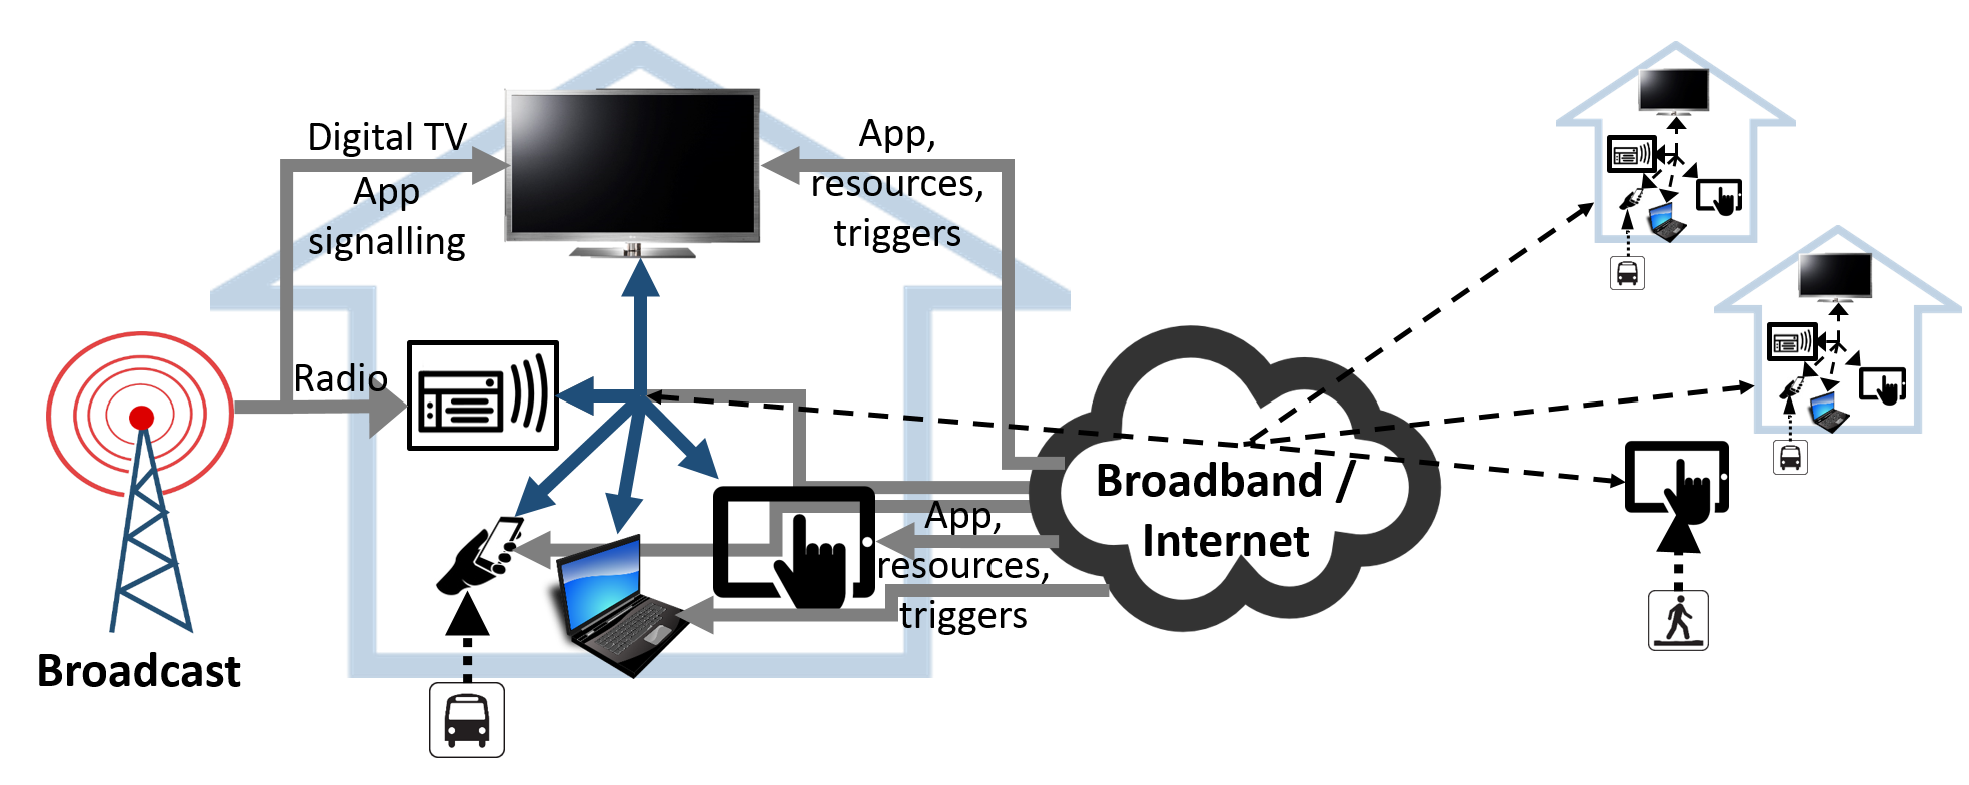
\includegraphics[width=0.75\textwidth]{General_Hybrid_cropped}
	\caption{General overview of the Hybrid TV and multi-device experiences \cite{Zorrilla2015}}
	\label{fig:hybrid}
\end{figure*} 
%
Several research projects have contributed to this field, such as the MediaScape \cite{MediascapeWeb} European FP7-ICT-2013-10 project, ended in May 2016, which focused its work on helping broadcasters and application developers to easily provide socially engaging media-driven experiences across multiple screens for hybrid broadcast-Internet content. MediaScape created open specifications and libraries on top of HTML5 and Web technologies, thus enabling the marriage of the TV, PC and Mobile worlds. The resulting libraries are based on the \textit{Created Once and Published Everywhere} (COPE) concept \cite{nem}. This means that the broadcaster will create a single application code, and the application itself will adapt to the multi-device environment of the user, providing association mechanisms, cross-device synchronisation and a dynamic self-regulated adaptation. 

Regarding the advantages of multi-screen systems, they enable broadcasters and application developers to provide their users with more content related to the mainstream media. They also offer opportunities for controlling the experience as well as for allowing the user to include new ways of personalisation, social sharing and consumption of media content from various sources \cite{cesar2008usages}. However, besides obvious advantages delivered by multi-screen media, more screens demand higher cognitive load for viewers to understand what they watch and to correlate content from different video streams. The required visual attention also increases and needs to be distributed across multiple displays situated at various locations in a three dimensional space \cite{vatavu2015evaluating}.

In this context, the user interface becomes a key factor in order to provide the users with a good experience across multiple devices at the same time, facilitating the understanding of the whole application and providing an intuitive interaction way. When broadcasters or application developers are facing a single-device user interface, they typically define a template to organise the items within a layout, usually describing different behaviours of the layout for disparate target devices. For instance, in Web applications developers can provide a CSS template with Media Queries that will adapt the user interface of the application to the final features of the device.

However, when developers are dealing with multi-device applications, this approach becomes unmanageable. Regarding multi-device adaptation, \cite{Zorrilla2015} provides a Web-based distributed adaptation architecture for media-driven multi-device applications, enabling broadcasters to provide the users with a single experience through multiple devices at the same time. In that solution, the system dynamically decides which elements of the application have to be shown on each device, splitting the application through different devices simultaneously, in order to provide a consistent and coherent view to the user. This means that the list of elements available on each device depends on the changing context of the users and will be updated dynamically when a new device is added or removed. In this scenario, it would be tedious, very expensive and unaffordable for developers to provide explicit rules to organise the elements on a user interface for all the possible combinations, and even more for each target device. The proposed multi-device adaptation solution in \cite{Zorrilla2015} provides arbitrary divisions to arrange the elements in a responsive user interface following some given rules, and creating a specific layout template according to the circumstances.

Nevertheless, it is still not easy for broadcasters and application developers to create a set of rules and hints to select the best user interface based on some contextual information, since they are not used to this. There are aspects in interface design, such as the functionality and usability that are well known aspects in the field of Human Computer Interaction (HCI), where the developers have stronger criteria \cite{mcnamara2006functionality}. For example, for a background device such as a TV, developers might want to allow overlaps between the different elements with Picture-in-Picture-like interfaces, while preventing elements to appear below the visible area of the screen to avoid scrolling. This pattern could be completely different for a touchable device, in the same way that it will be very dependant on the nature of the media application and its elements. Moreover, in addition to the traditional HCI parameters, there is a new wave in the field emphasising the importance of aesthetic aspects in interface design for the users’ likability and system acceptability \cite{bauerly2008effects} \cite{altaboli2011investigating}.

In this context, the discussion of the user interface elements and design factors that are involved in a multi-device media application could become a valuable research. On the one hand, all the considered dimensions could contemplate the functionality, usability and aesthetic aspects addressed in the literature for single-device interface design. On the other hand, the factors should contemplate the new interface design aspects introduced by the multi-device dimension, not yet addressed in the literature, as one main contribution of this work. Furthermore, it would be desirable to provide a user interface model for media applications in multiple devices simultaneously, on top of the user interface elements and design factors previously defined. This model would aim to be as general and flexible as possible, for it to be parametrised by developers according to the needs of the specific application and over well-known HCI concepts. From these HCI criteria parametrisation, the general model could conclude in an automatically created set of rules to be applied in a multi-screen system, and the rules would decide the distribution of the content across the connected devices and the layout templates according to the specific contextual information of the multi-device dimension.



\section{Hypothesis}\label{hypothesis}

The interoperable and standard-based solution presented in \cite{thesisMikel} fosters the broadcast-Internet convergence and allows broadcasters and media application developers to easily create applications on top of the COPE concept. In this context, the working hypothesis is constructed as a statement of the following expectations:

\begin{enumerate}
			
	\item It is possible to define a general methodology that will end with an adaptation model to seamlessly adapt the user interface of multi-device media services.

		\begin{enumerate}
			\item A large-scale pilot deployment of a hybrid broadcast-Internet multi-device service for a live TV programme on top of the Web-based distributed architecture presented in \cite{Zorrilla2015} could provide very valuable knowledge regarding the experience with the broadcaster, the application development and the end user usage of the service.
			\item With the learnt lessons an overall methodology which faces the muti-device adaptation taking into account a wide range of design factors could be defined.
			\item The methodology will end in a model able to both distribute the content across devices and generate a layout template for each connected device.
			\item The model could provide a near real-time adaptation while guaranteeing a good quality.
			\item The model may need to be iterative in order to take into account the context information mainly produced by the user but also related to environmental and system factors. 
			\item The model could be complemented with learning processes that allow to modify or refeed it with context information.		
		\end{enumerate}
	\item This methodology will be adaptable and extensible to other application fields, adjusting to the specific requirements of each case:
	
	\begin{enumerate}
		\item It could be general enough to be extended to any type of content or device and also ready for technological changes.
		\item It could be used in different scenarios and use cases within the broadcast field such as the ones shown in Figure \ref{fig:scenarios}
		\item It could be useful for other sectors where multiple devices are used at the same time, such as Industry 4.0 or crisis management environments where the role of videowalls could be relevant.
	\end{enumerate}
	
	\begin{figure}
		\centering
		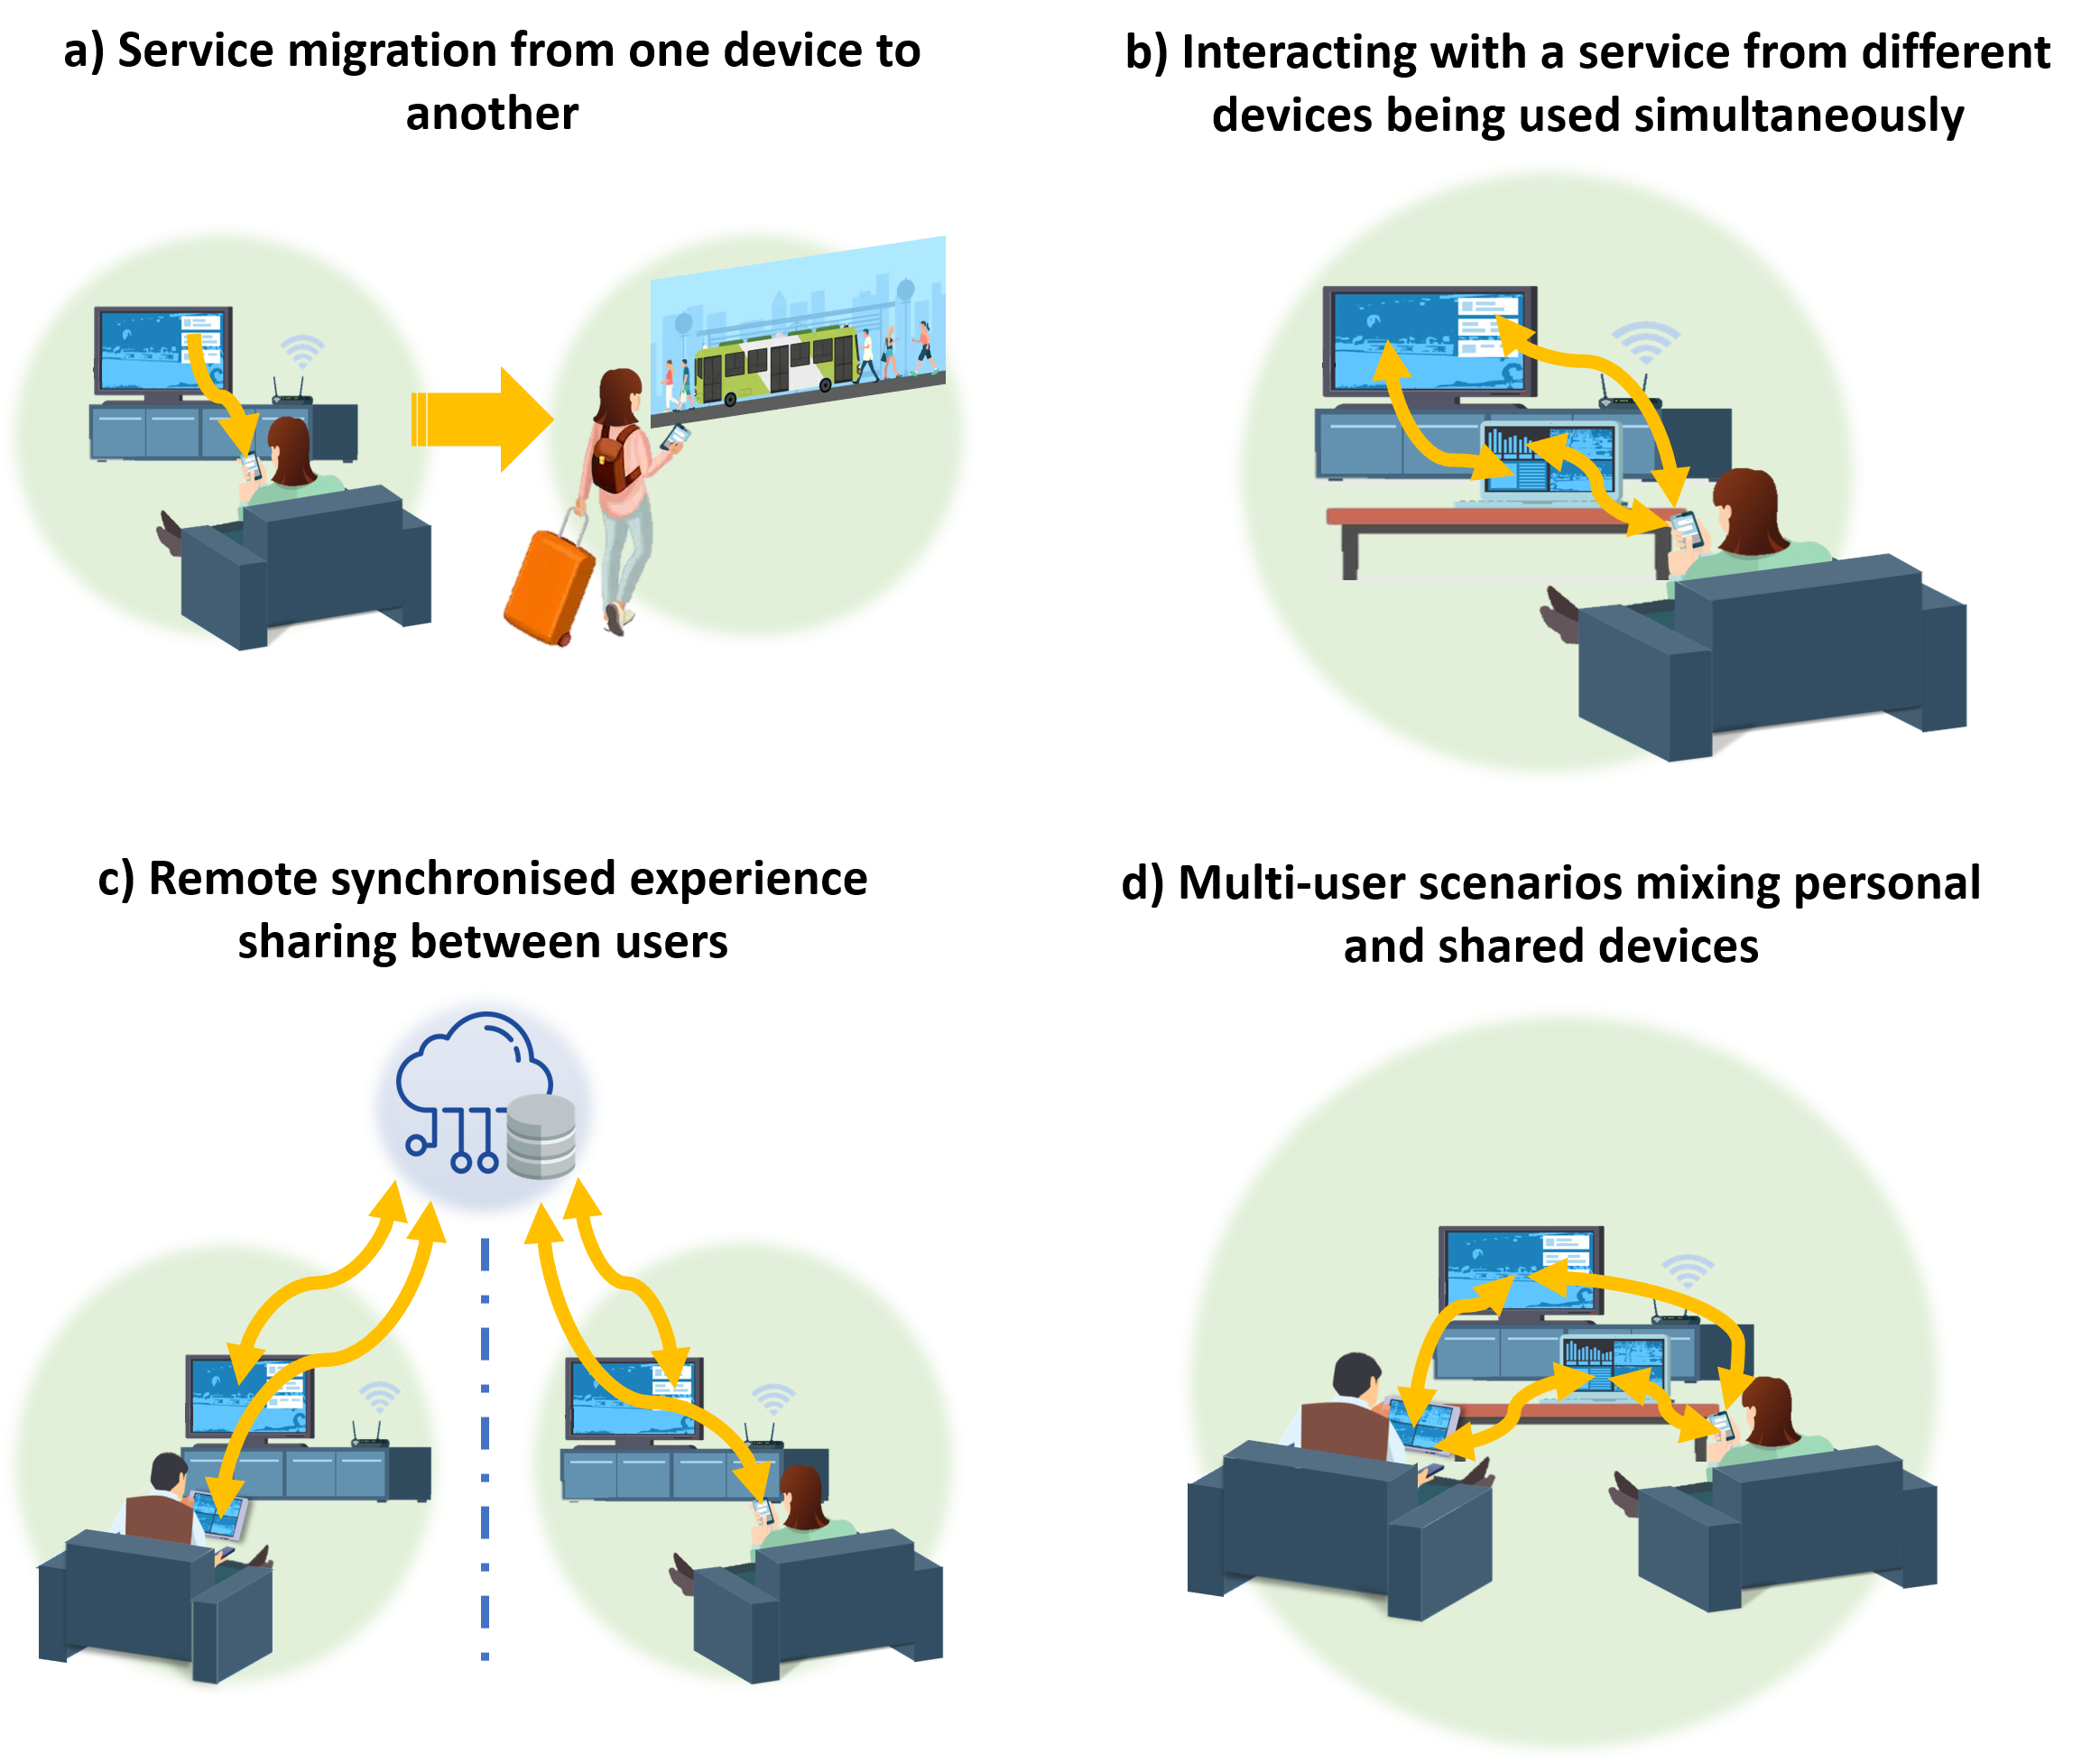
\includegraphics[width=1\textwidth]{scenarios.png}
		\caption[Different multi-device scenarios which could be found in the broadcast field]{Different multi-device scenarios which could be found in the broadcast field}
		\label{fig:scenarios}
	\end{figure}
	
\end{enumerate}

\section{Objectives}\label{objectives}
The main objective of this work is to provide a methodology which provides as an outcome an adaptation model for the user interface of multi-device media services, general enough to be easily adapted to many different use cases and scenarios and ready for any technological update. In order to reach that goal it is necessary to overcome the following challenges:

\begin{itemize}
	\item Objective 1: Generate a real pilot deployment of a hybrid broadcast-Internet multi-device service for a live TV programme using a rule-based adaptation process that allows to draw some conclusions in order to face the definition of a general adaptation model for the user interface of multi-device media services. \label{objective:1}	
	\item Objective 2: Define a methodology that goes an step further than explicit adaptation rules and allows to generate more automatic and simple adaptation models for applications based on the COPE (Create Once and Publish Everywhere) \cite{nem} concept and the trend of componentizing the Web \cite{savage2015componentizing}. In addition, the objective behind the methodology is to ease developers and broadcasters the creation of seamless and self-adaptive applications.\label{objective:2}	 
	\item Objective 3: Define a flexible and extensible adaptation model in such a way that it is still good not only for every use case, scenario and technological change but also for other sectors different from the broadcast. For that, it will be necessary to identify and characterise several user interface elements and design factors, but the methodology will conclude on an adequate model given a specific context.\label{objective:3}	
	\item Objective 4: Provide example implementations in order to validate the methodology and the model in terms of quality, efficiency, adaptability, flexibility and extensibility.\label{objective:4}	
	
\end{itemize}  
\section{Methodology}\label{methodology}

The research work performed in this Ph.D. has followed a methodology based on the two loop design cycle described in Figure \ref{fig:designcycle}. 
\begin{figure}
	\centering
	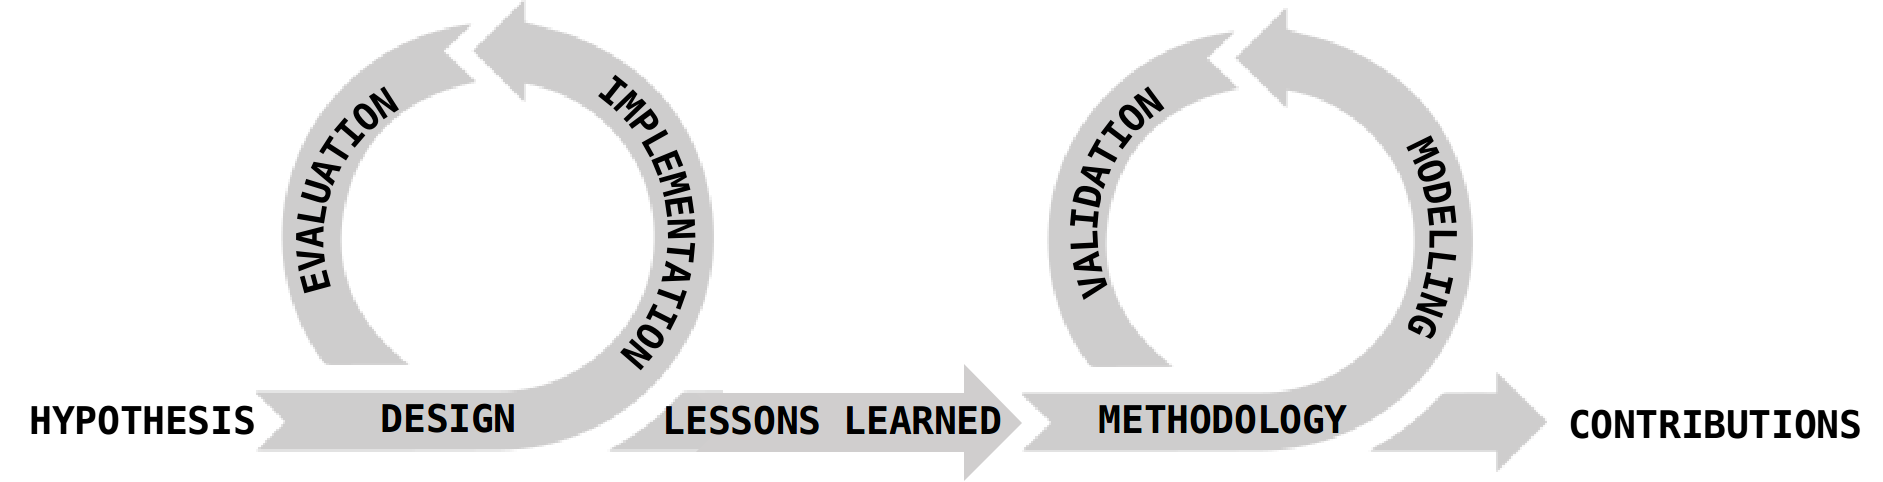
\includegraphics[width=1\textwidth]{methodology.png}
	\caption[Design cycle followed as the research methodology]{Design cycle followed as the research methodology}
	\label{fig:designcycle}
\end{figure}
Based on the motivation for this research topic, a working \textbf{hypothesis} has been constructed as a statement of expectations. To achieve the two main \textbf{contributions} of the research, a two stage procedure has been followed: 

On the first stage, a real pilot deployment of a hybrid broadcast-Internet multi-device service has been designed, implemented and evaluated: 
\begin{itemize}
	\item \textbf{Design}: First of all, the design objectives have been clearly defined to be addressed during the architectural design of the different aspects of the solution.
	\item \textbf{Implementation}: A real pilot has been implemented following the architectural design and the guidelines of a broadcaster.
	\item \textbf{Evaluation}: The deployment has been evaluated providing the developed service to the audience and analysing the usage statistics of more than a thousand users.
\end{itemize}

Once the first stage has been completed the hypothesis has been adjusted taking into account the lessons learned from the previous deployment. Then, a second stage has been carried out in which a methodology has been defined to generate adaptation models for multi-device media services general enough to be ready for  every use case as well as for every technological change. For that, this second stage has been divided into three steps:

\begin{itemize}
	\item \textbf{Methodology}: A methodology has been defined with different steps, to gather information that allows to identify all the elements and design factors that play an important role in the adaptation process of a multi-device user interface. 
	\item \textbf{Modelling}: Taking into account all the information gathered along the steps of the previous methodology, a model has been defined which includes the characterisation of the involved user interface elements, the adaptation process and an evaluation model.
	\item \textbf{Validation}: Implementation examples of the model have been developed in order to validate its quality, efficiency, adaptability, flexibility and extensibility. 
\end{itemize}


The two stage procedure has helped to refine the design and implementation of the target solution, leading to the final contributions of the research.



\section{Contributions}\label{contributions}
The main contribution of this Ph.D. research has been the definition of an adaptation model for the user interface of multi-device media services, general enough to be easily adapted to many different use cases and scenarios and ready for any technological update. As a result of the objectives mentioned in Section \ref{objectives} the main contribution can be translated into three specific outcomes: 
\begin{enumerate}
	\item Design and implementation of a large-scale deployment of a hybrid broadcast-Internet multi-device service for a live TV programme which shows the lessons learned about the current hybrid broadcast-Internet ecosystem and multi-device live services. \label{contribution:1}
	\item Design and implementation of a methodology that provides as an outcome an adaptation model for the user interface of multi-device media services, which has been formally described and validated in terms of quality, efficiency and universality. This includes the identification and characterisation of all the user interface elements involved in the adaptation process. \label{contribution:2}
	\item Identification of different fields in which the proposed methodology could be applicable.\label{contribution:3}
	
\end{enumerate}

\begin{figure}
	\centering
	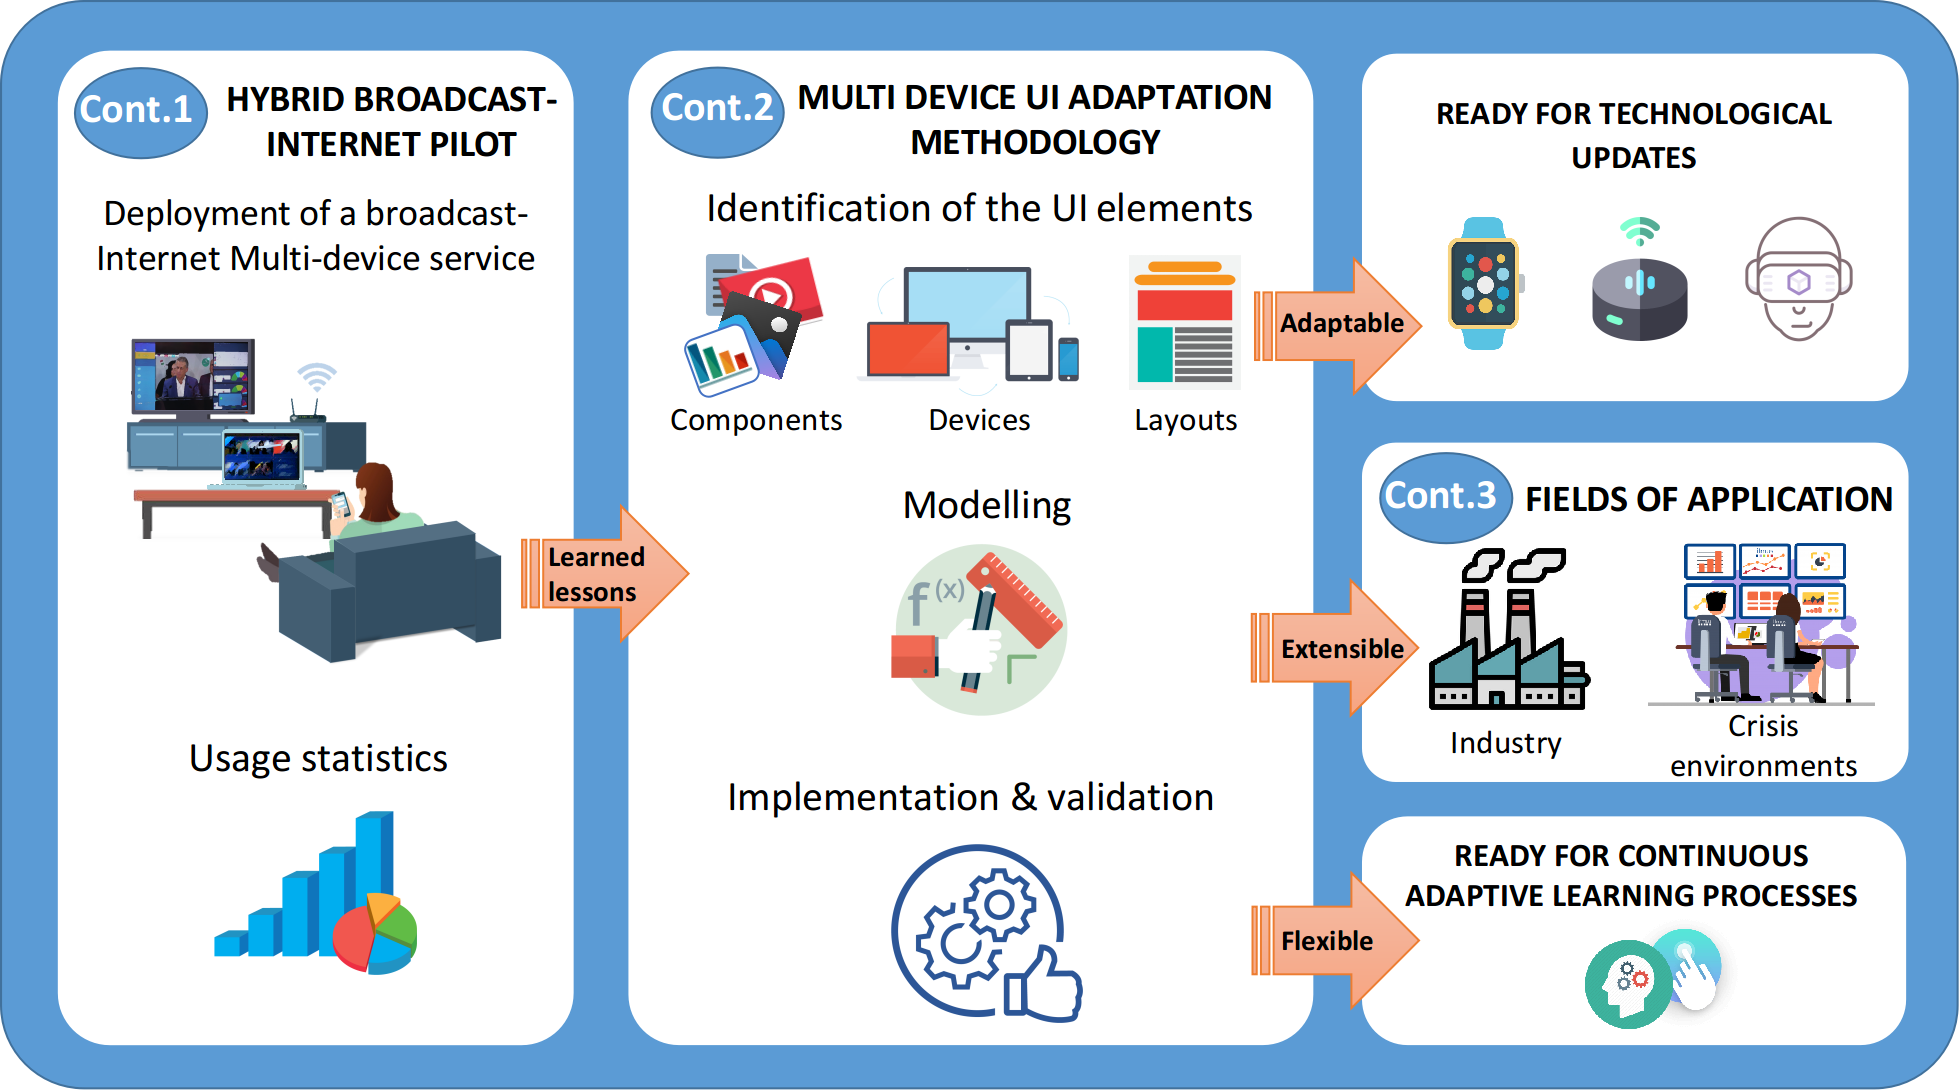
\includegraphics[width=1\textwidth]{PhdContributions1.png}
	\caption[Contributions of the research]{Contributions of the research}
	\label{fig:PhdContributions}
\end{figure}

Figure \ref{fig:PhdContributions} illustrates the three contributions of the research to address the definition of an adaptation model for the user interface of multi-device media services. Furthermore, it shows the readiness of the model to be adapted to technological updates as well as to be integrated with continuous adaptive learning processes. 

\begin{figure}
	\centering
	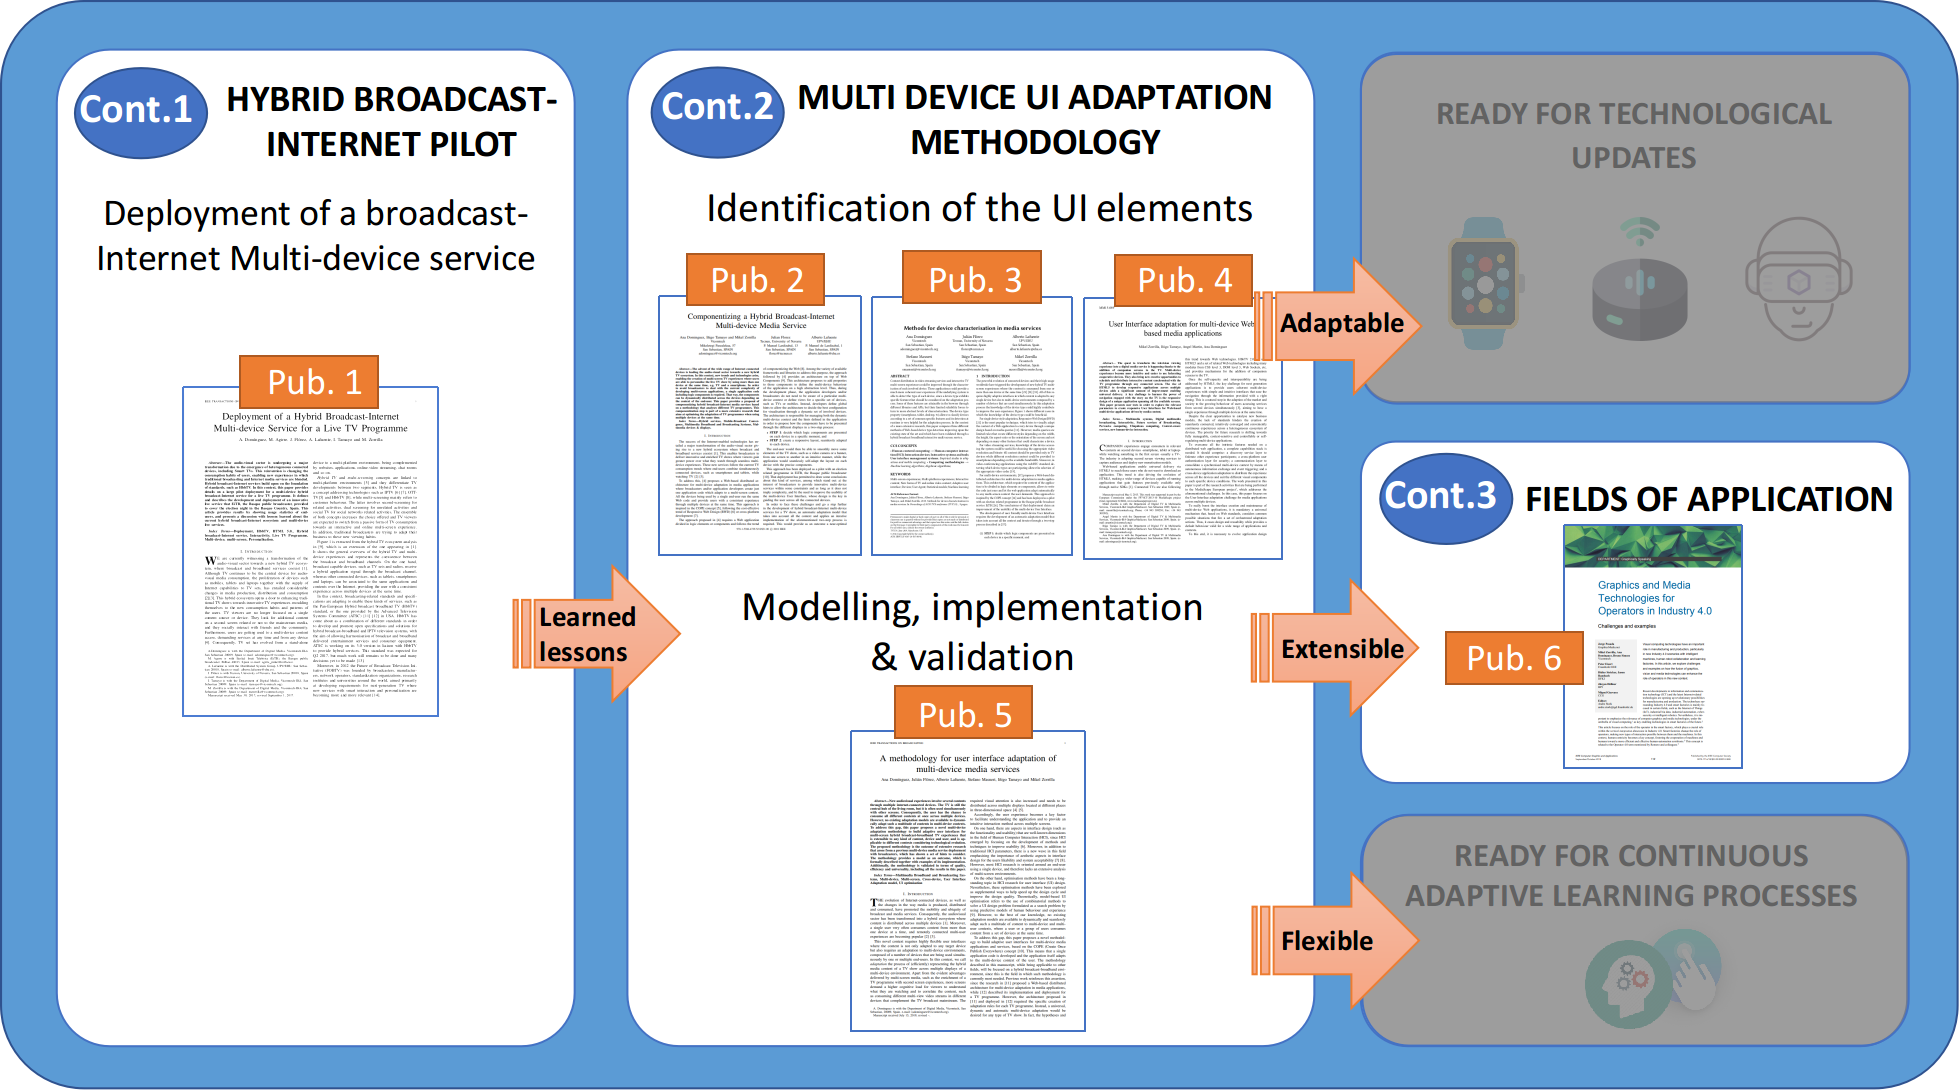
\includegraphics[width=1\textwidth]{PhdContributions2.png}
	\caption[Publications of the research]{Publications of the research}
	\label{fig:PhdPublications}
\end{figure}

The contributions delivered the following publications:
\begin{itemize}
	\item Publications related to Contribution \ref{contribution:1}:
	\begin{itemize}
		\item Pub. 1: \textit{Dominguez, A., Agirre, M., Flörez, J., Lafuente, A., Tamayo, I., \& Zorrilla, M. (2017). Deployment of a hybrid broadcast-Internet multi-device service for a live TV programme. IEEE Transactions on Broadcasting, 64(1), 153-163.}
	\end{itemize}
	\item Publications related to Contribution \ref{contribution:2}:
	\begin{itemize}
		\item Pub. 2: \textit{Dominguez, A., Tamayo, I., Zorrilla, M., Flórez, J., \& Lafuente, A. (2018, June). Componentizing a Hybrid Broadcast-Internet Multi-device Media Service. In 2018 IEEE International Symposium on Broadband Multimedia Systems and Broadcasting (BMSB) (pp. 1-6). IEEE.}
		\item Pub. 3: \textit{Dominguez, A., Florez, J., Lafuente, A., Masneri, S., Tamayo, I., \& Zorrilla, M. (2019, June). Methods for device characterisation in media services. In Proceedings of the 2019 ACM International Conference on Interactive Experiences for TV and Online Video (pp. 118-128). ACM.}
		\item Pub. 4: \textit{Zorrilla, M., Tamayo, I., Martin, A., \& Dominguez, A. (2015, June). User interface adaptation for multi-device Web-based media applications. In 2015 IEEE International Symposium on Broadband Multimedia Systems and Broadcasting (pp. 1-7). IEEE.}
		\item Pub. 5: \textit{Dominguez, A., Florez, J., Lafuente, A., Masneri, S., Tamayo, I., \& Zorrilla, M. (Submitted in 2019, November). A methodology for user interface adaptation of multi-device media services. IEEE Transactions on Broadcasting.}
	\end{itemize}
	\item Publications related to Contribution \ref{contribution:3}:
	\begin{itemize}	
		\item Pub. 6: \textit{Posada, J., Zorrilla, M., Dominguez, A., Simoes, B., Eisert, P., Stricker, D., Rambach, J., Döllner, J. \& Guevara, M. (2018). Graphics and media technologies for operators in industry 4.0. IEEE computer graphics and applications, 38(5), 119-132.}
	\end{itemize}
	
\end{itemize}

Figure \ref{fig:PhdPublications} shows the relation between the objectives, the contributions and publications. 


\section{Document structure}

This thesis has been structured as follows. Part \ref{sec:Part1} presents an introduction to the research scope, focusing on the motivation for the research, the main objectives, the hypothesis, the methodology and the main contributions of the Ph.D. work. 

Part \ref{sec:Part2} overviews literature related to the hybrid ecosystem, the involved specifications and technologies in ubiquitous media applications and the adaptation and optimisation of the user interface of web applications.

In Part \ref{sec:Part3} the research results are described in three main chapters:

\begin{itemize}
	\item Chapter \ref{chap:deployment} describes the deployment of a large-scale pilot of a hybrid broadcast-Internet multi-device service for a live TV programme and the lessons learned (Contribution \ref{contribution:1}).
	\item Chapter \ref{chap:adaptation} describes a methodology that enables to generate an adaptation model for multi-device media services together with its implementation and validation (Contribution \ref{contribution:2}).
	\item Chapter \ref{chap:fields} describes how the proposed methodology could be applicable in other fields beyond broadcast (Contribution \ref{contribution:3}).
\end{itemize}


In Part \ref{sec:Part4} the main conclusions of the research can be found, including a discussion that enables future work.

Finally, Part \ref{sec:appendix} provides the Curriculum Vitae of the author as an appendix, while Part \ref{sec:bibliography} contains the bibliography.
